\section{Durchführung}
\label{sec:Durchführung}
Im Folgenden wird beschrieben, wie ein Diodenlaser in Betrieb genommen wird und wie das Absorptionsspektrum von Rubidium aufgenommen wird.
\subsection{Versuchsaufbau}
Zunächst muss der Diodenlaser an eine Stromquelle angeschlossen werden. Zusätzlich müssen 2 Photodetektoren mit Strom versorgt werden und 
an ein Oszilloskop angeschlossen werden. Der Diodenlaser wird auf einen optischen Tisch montiert und die optischen Elemente so justiert, dass
der Laserstrahl auf die Rubidiumdampfzelle fällt. Bei der hier verwendeten Methode der Absorptionsspektoskopie wird der Laserstrahl aufgespalten
und ein Teil des Strahls wird durch die Rubidiumdampfzelle geschickt. Der andere Teil wird direkt detektiert. Die Differenz der detektierten Intensität 
gibt nun Auskunft wie vie Licht Absorbiert wird. Wird die Wellenlänge des Lasers nun leicht verändert, so kann das Absorptionsspektrum aufgenommen werden.
Die Verschaltung ist in Abbildung \ref{fig:versuchsaufbau} dargestellt. Der Aufbau der optischen Elemente ist in Abbildung \ref{fig:optische_elemente} dargestellt.
Für die Spektroskopie wird infrarot Licht verwendet, welches nicht sichtbar ist. Deshalb wird eine CCD-Kamera verwendet, um das Spektrum sichtbar zu machen.
Zum Schutz vor der unsichtbaren, aber wegen der hohen Intensität nicht minder gefährlichen Strahlung wird während des gesamten Versuchs eine Schutzbrille getragen.
\begin{figure}[H]
    \centering
    \includegraphics[width=0.7\textwidth]{pictures/Aufbau.JPG}
    \caption{Verschaltung der elektronischen Bauteile}
    \label{fig:versuchsaufbau}
\end{figure}
\begin{figure}[H]
    \centering
    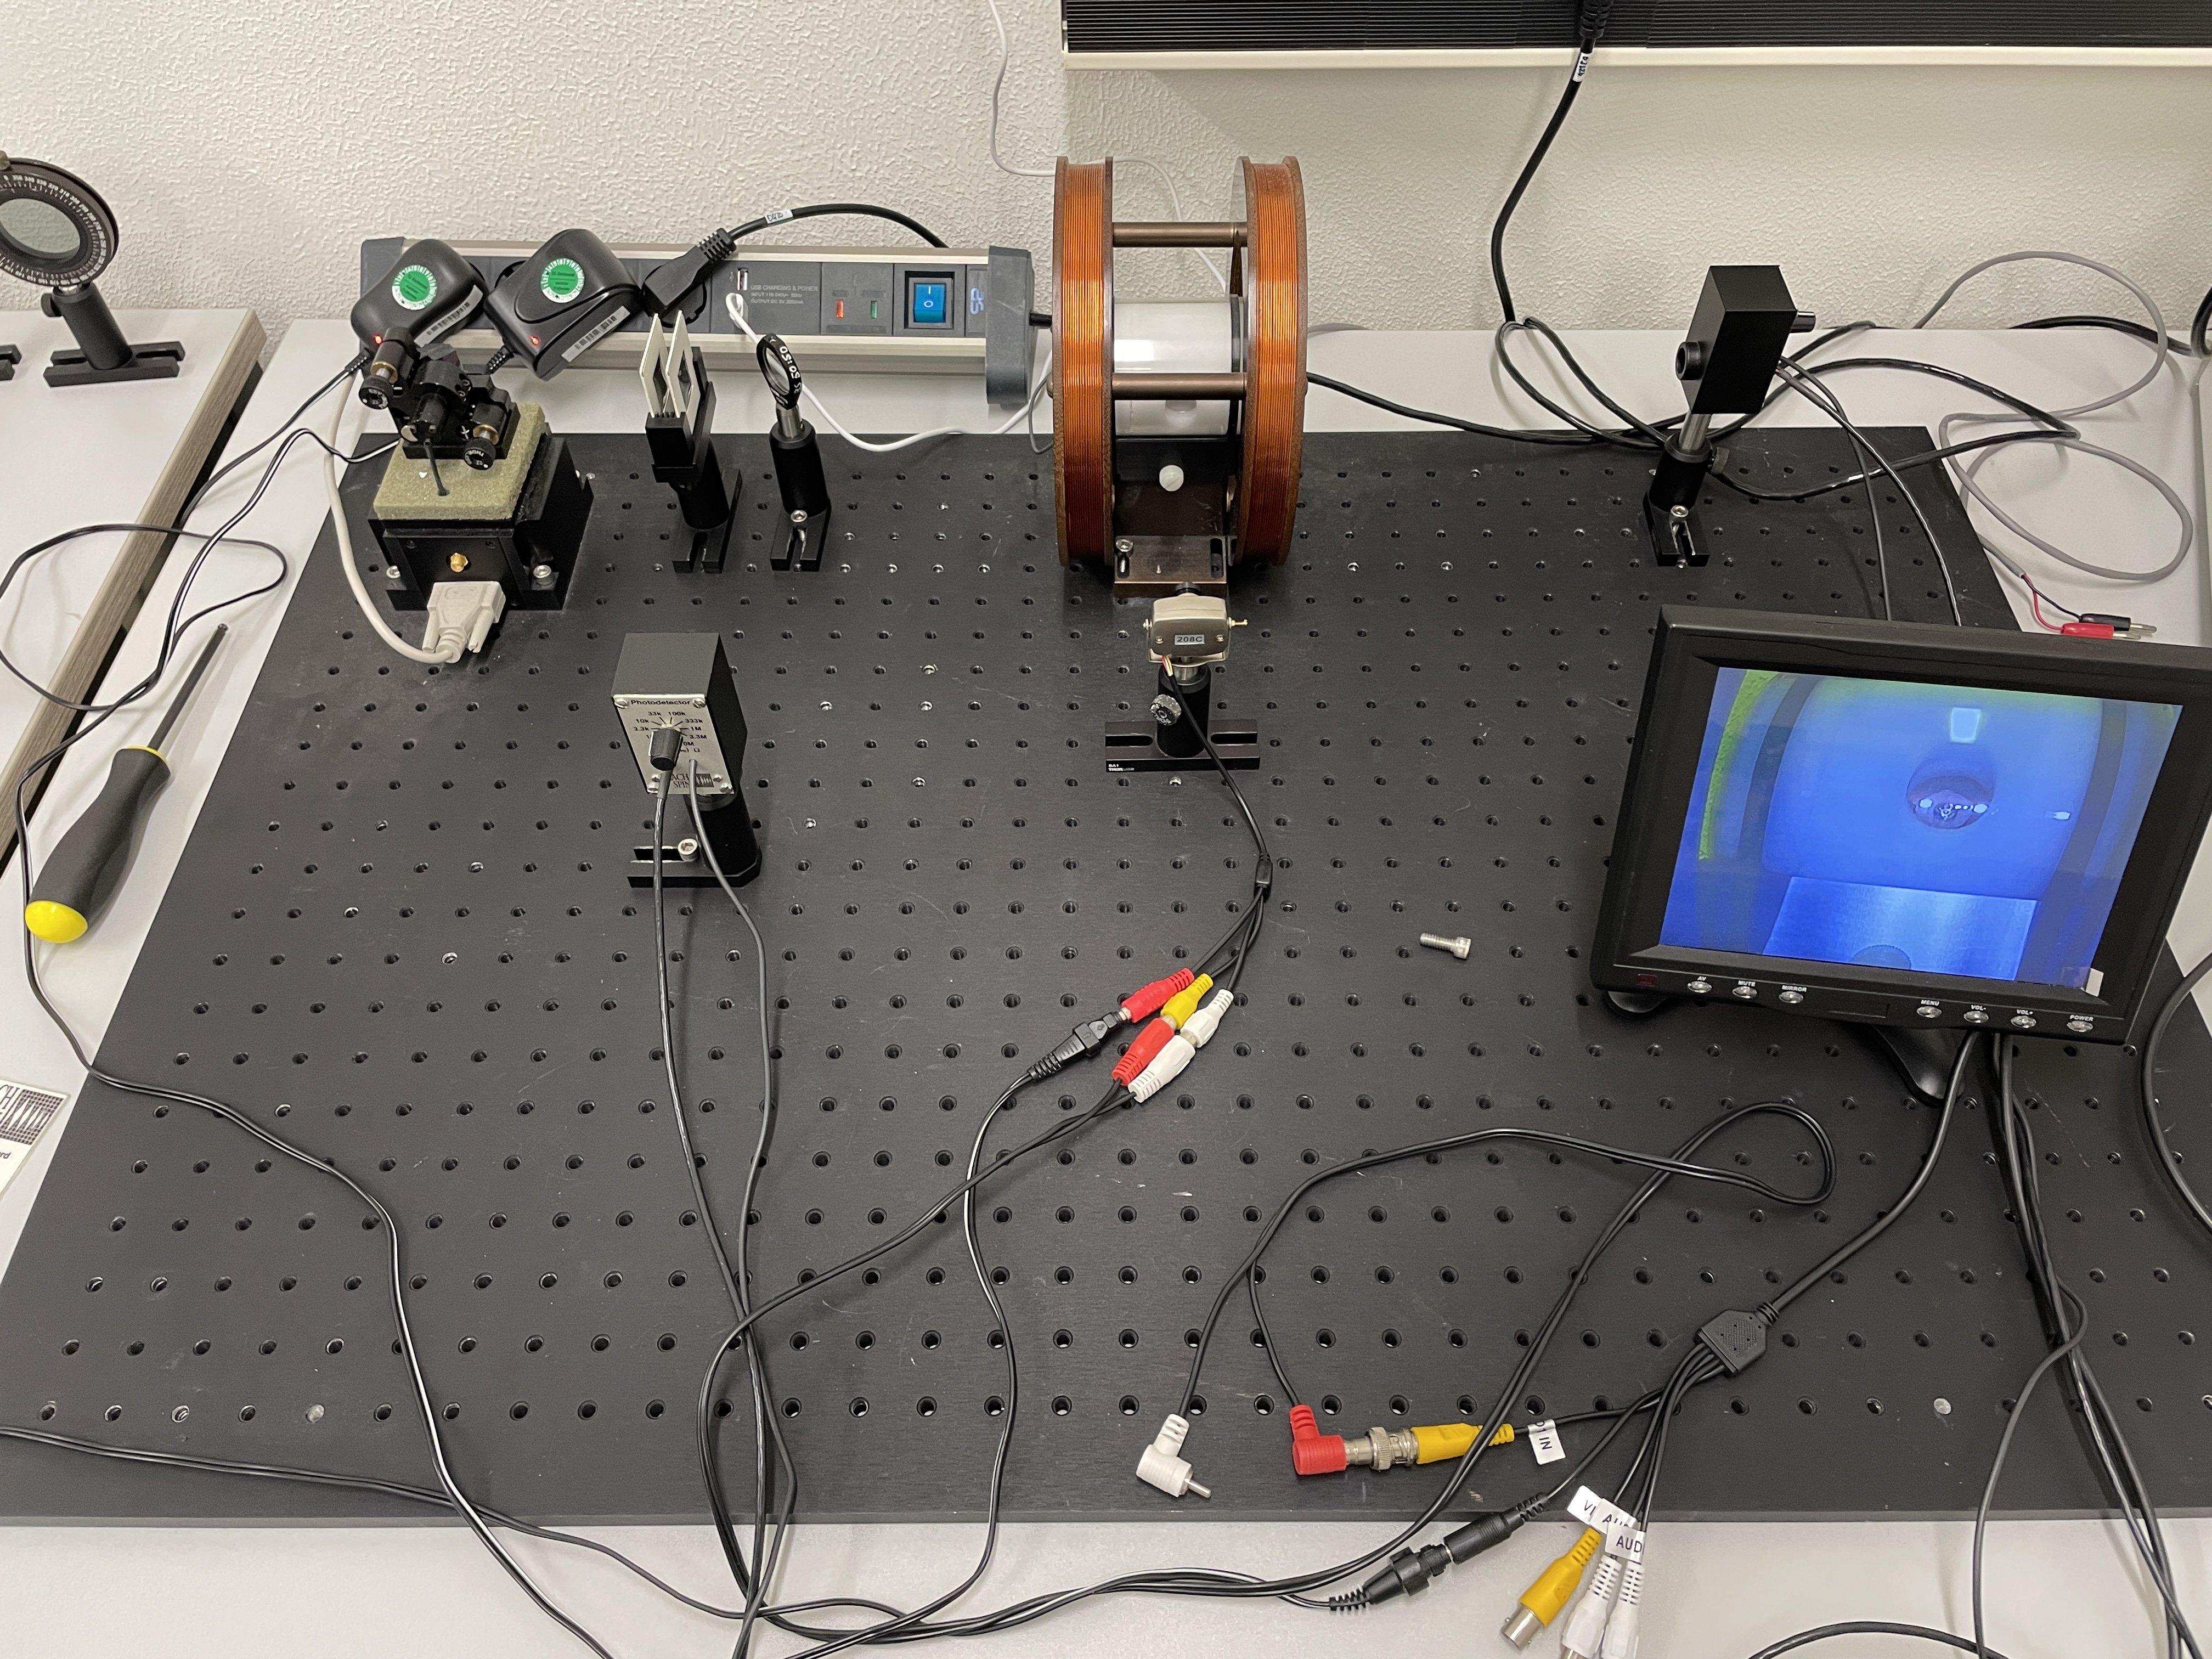
\includegraphics[width=0.7\textwidth]{pictures/Aufbau2.JPG}
    \caption{Platzierung der optischen Elemente auf dem optischen Tisch}
    \label{fig:optische_elemente}
\end{figure}
\subsection{Versuchsablauf}
Die erste Aufgabe besteht darin den Diodenlaser in Betrieb zu nehmen. Dazu werden alle elektronischen Bauteile angeschlossen und eingeschaltet.
Nun muss der Schwellstrom bestimmt werden, ab dem die Diode vom LED Betrieb in den Laserbetrieb übergeht. Dazu wird der Strom langsam erhöht und ein Indikatorpapier 
für Infrarotstrahlung in den Strahl gehalten. Sobald der Laser in Betrieb geht, wird die Intensität größer, aber wegen der kohärenten Natur des Lichts 
lassen sich auf der Oberfläche des Indikators am Rand Anzeichen eines Interferenzmusters erkennen. Es wird ein Photo zum Vergleich gemacht und der Schwellstrom notiert.
Nun werden auch die optischen Bauelemente so auf der Bank paltziert. Mit dem Indikator kann geprüft werden, ob der Strahl richtig verläuft oder 
ob die Elemente etwas gedreht werden müssen. Ist der Strahl richtig justiert, so wird die Rubidiumdampfzelle mit einer CCD-Kamera beobachtet.
Am Laser wird nun ganz leicht der Winkel des Gitters verändert, sodass die Wellenlänge des Lasers leicht verändert wird. Wenn die Absorptionswellenlänge 
des Rubidiums getroffen wird, so fängt das Rubidiumgas an zu fluoreszieren.

\noindent Nun kann der Sweep so eingestellt werden, dass das ganze Spektrum aufgenommen wird. Die Photodetektoren werden so zueinander eingestellt, dass wenn nichts absorbiert wird,
das Oszilloskop eine gerade Linie anzeigt. Wenn der Sweep so eingestellt ist, dass kein Mode Hoping auftritt, kann das Signal verstärkt werden und aufgenommen werden. 
Die Peaks entsprechen den Absorptionsminima.